% -*- mode: latex; mode: flyspell -*-

%%% Local Variables:
%%% TeX-master: "mu2e-36575"
%%% End:

%%%%%%%%%%%%%%%%%%%%%%%%%%%%%%%%%%%%%%%%%%%%%%%%%%%%%%%%%%%%%%%%%%%%%%%%%%%%%%
\section{Particle Identification}

Momentum region around 100 MeV/c muons is withing the range where transition from non-relativistic
to ultra-relativistic regime is happening for muons. As shown in Figure \ref{fig:pid_ep_dt}
distributions of important for particle ID variables for 92 MeV/c and 105 MeV/c muons are quite
different. Therefore it makes sense to optimize the particle ID algorithms for \MuToEm\ and \MuToEp\ 
conversion searches separately.

\begin{figure}[H]
\hspace{-0.6in}
  \begin{tikzpicture}
    \node[anchor=south west,inner sep=0] at (0,0.) {
      % \node[shift={(0 cm,0.cm)},inner sep=0,rotate={90}] at (0,0) {}
      % \makebox[\textwidth][c] {
      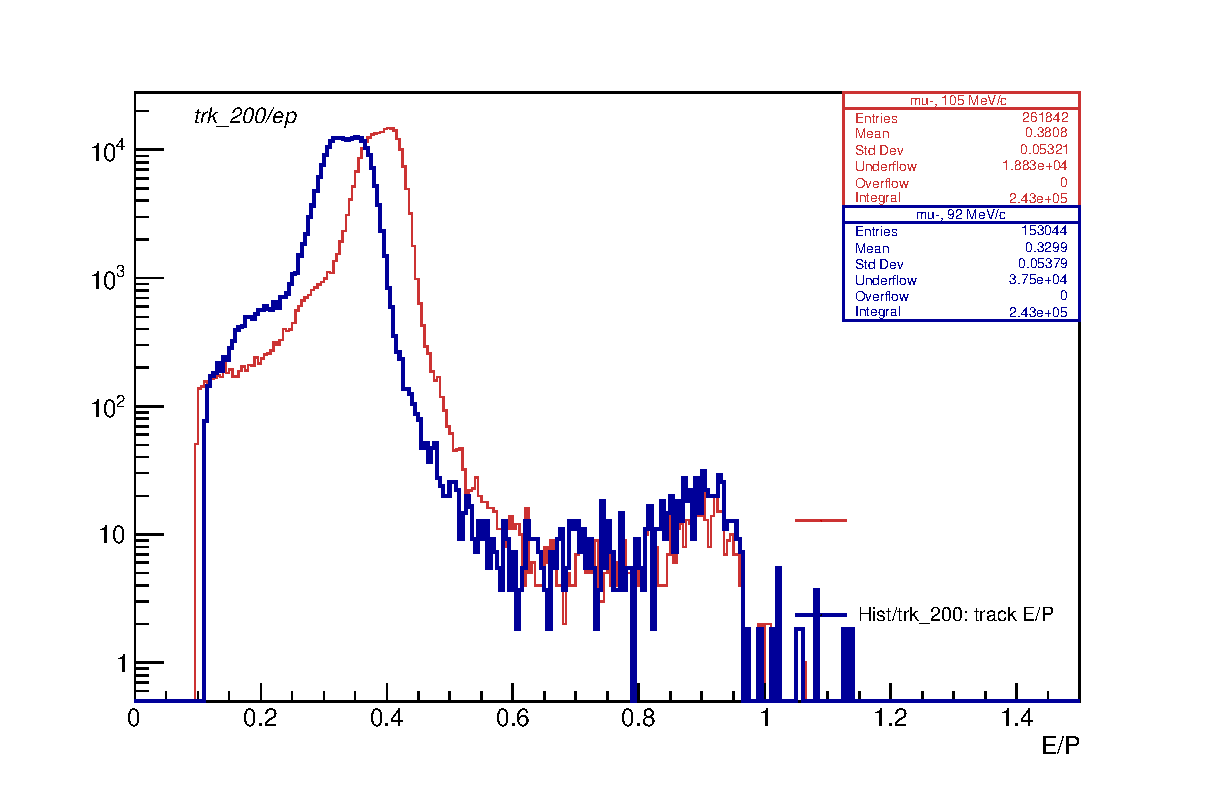
\includegraphics[width=0.64\textwidth]{figures/pdf/figure_00321_su2020_track_ana_trk_200_ep}
      % }
    };
    \node[anchor=south west,inner sep=0] at (10.5,0.) {
      % \node[shift={(0 cm,0.cm)},inner sep=0,rotate={90}] at (0,0) {}
      % \makebox[\textwidth][c] {
      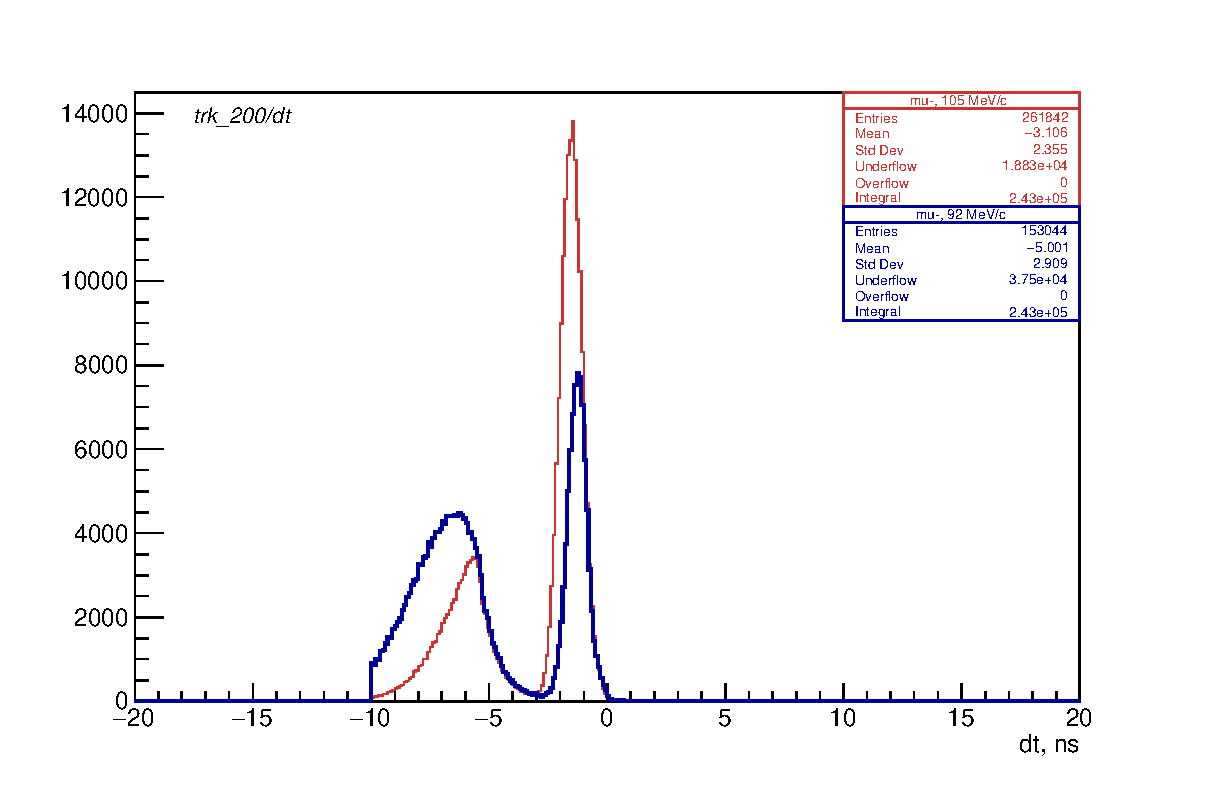
\includegraphics[width=0.64\textwidth]{figures/pdf/figure_00322_su2020_track_ana_trk_200_dt}
      % }
    };
    % \node [text width=6cm, scale=0.8] at (4.5,6.4) {mu2e-18894 by Kevin Lynch and Jim Popp};
  \end{tikzpicture}
  % \captionof{figure} {
  \caption{
  \label{fig:pid_ep_dt}
    E/P and $\Delta T$ distributions for 105 and 92 MeV/c muon tracks reconstructed under electron
    hypothesis. Bump in between -10 and -5 ns in the $\Delta T$ distributions corresponds to events 
    with the calorimeter cluster rejected by the track fit, so the track T0 is not biased by the fit.
    Events in the peak around -1.5 ns have the ``track cluster hist'' surviving the fit and thus
    biasing the fit results.
  }
\end{figure}

There is an indication that the bias resulting from the inclusion of the calorimeter cluster
into the track fit somewhat degrades the separation between electrons and muons.
%
At the same time, inclusion of the cluster into the track fit stabilizes the track fit, improves its
convergence and, overall, results in a higher track reconstruction efficiency.
%
Taking both considerations into account, we've chosen to use ANN-based PID classifiers,
expecting the ANN training to ``absorb'' existing systematic effects while providing sufficiently
high level of muon rejection.

Single particle datasets {\bf ele00s61b0} and {\bf mumi0s61b0},  105 MeV/c electrons and$\mu^-$'s,
have been used to train the PID ANN for \MuToEm\ channel.

%%%%%%%%%%%%%%%%%%%%%%%%%%%%%%%%%%%%%%%%%%%%%%%%%%%%%%%%%%%%%%%%%%%%%%%%%%%%%%
\subsection {PID ANN Training }
\label{sec:mumem_pid_ann_training}

MVA classifiers were trained only for DAR resolver, however based on the nature of 
the variables used, the trained MVA should perform equally well for PAR tracks.

Both electron and muon reconstruction were ran on the same event. In principle, using 
for a given event information from two reconstruction passes adds information and may
improve electron-muon separation. However, it was found that adding requirement for each
track to be reconstructed under electron and muon hypotheses complicates logic and increases
the number of special cases to consider without providing a visible improvement. Therefore,
inputs for the ANN training are provided by the electron reconstruction only.

Events used for ANN training were required to have a downstream DAR track passing
the track selection cuts described in Section \ref{sec:track-selection_cuts_summary}.
%
The following event variables have been used in the ANN training:

\begin{itemize}
\item 
  {\bf E(cluster)/P(track)} : although all tracks used in training have the same generated momentum,
  using E/P reduces dependence on the track momentum 
\item 
  {\bf N(crystals)} : number of crystals in the reconstructed calorimeter cluster
\item 
  {\bf eSeedfr} : fraction of energy in the seed crystal ($E_{seed}/E_{cluster}$)
\item 
  {$\bf \Delta T$} : time residual of the calorimeter cluster as determined by the kalman fit
\item 
  {$\bf Z_{cluster}$} : cluster Z-coordinate (within the corresponding calorimeter disk) as determined by the kalman fit
\item 
  {$\bf \Delta R$} : radial residual of the calorimeter cluster as determined by the kalman fit
\item 
  {\bf path} : overall length of the trajectory within the calorimeter disk, defines edges
\end{itemize}

PID ANN training performed using ROOT TMVA package uses 10000 electron and 10000 muon events.
Events with muon decays in flight are excluded by requiring the last point (StepPointMC)
of the muon MC trajectory to have Z > 11000 mm.
%
To ensure that all event variables used in the ANN training are defined, events used for training
are required to pass the following requirements, the PID pre-selection cuts:

\begin{itemize}
\item 
  reconstructed under electron hypothesis track passes the track selection cuts
\item 
  an event has a reconstructed cluster 
\item 
  $\Delta T > -100$ : this is a requirement for the calorimeter cluster not to be rejected by the track fit.
  Ff the cluster is rejected, the $\Delta T$ value set to -999.
\item
  $-50 mm ~<~ Z_{cluster} ~<~ 250 mm$ : after the fit, the cluster Z coordinate is consistent in Z with the
  Z-position of the corresponding calorimeter disk. 
\end{itemize}

Figures \ref{fig:pid_training_1} and \ref{fig:pid_training_2} show distributions of the electron
and muon variables used for ANN training.

\begin{figure}[H]
  \hspace{-0.6in}
  \begin{tikzpicture}
    \node[anchor=south west,inner sep=0] at (-1,0.) {
      % \node[shift={(0 cm,0.cm)},inner sep=0,rotate={90}] at (0,0) {}
      % \makebox[\textwidth][c] {
      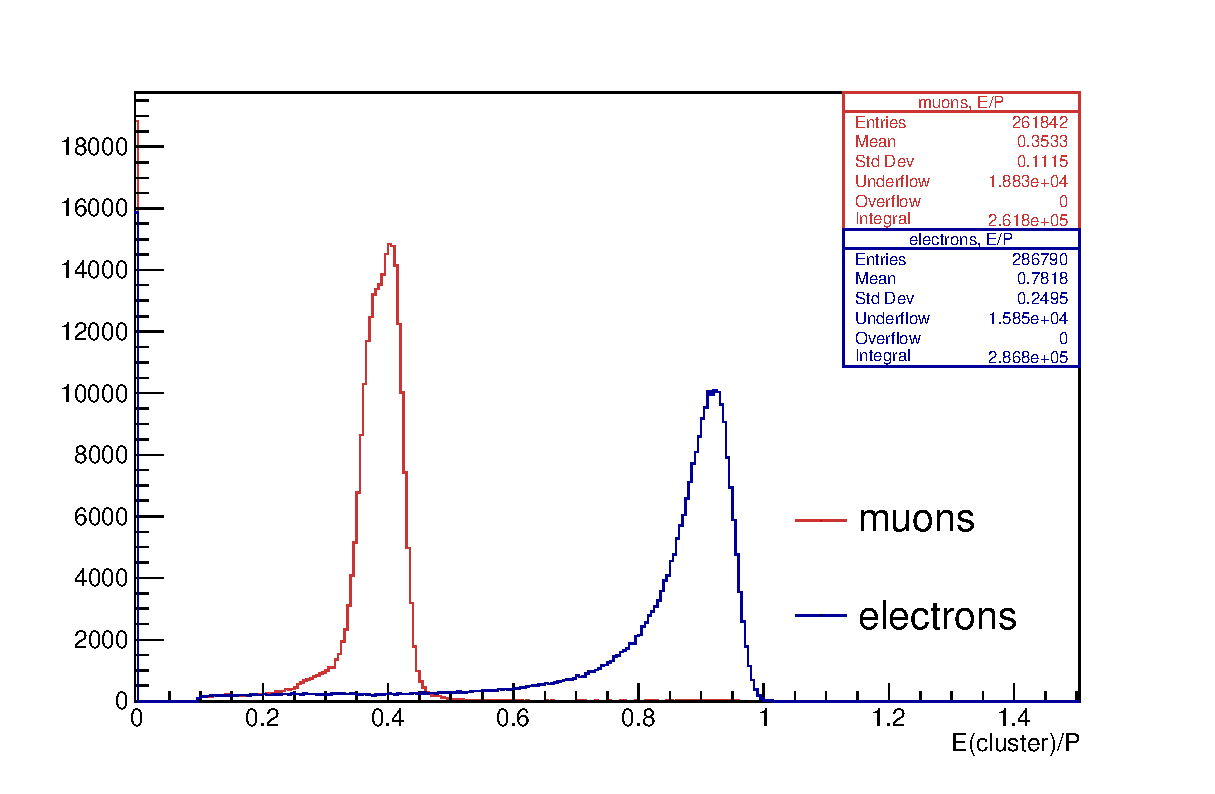
\includegraphics[width=0.50\textwidth]{figures/pdf/figure_00300_pid_emuana_1070_trk_101_ep}
    % }
    };
    \node[anchor=south west,inner sep=0] at (9.5,0.) {
      % \node[shift={(0 cm,0.cm)},inner sep=0,rotate={90}] at (0,0) {}
      % \makebox[\textwidth][c] {
      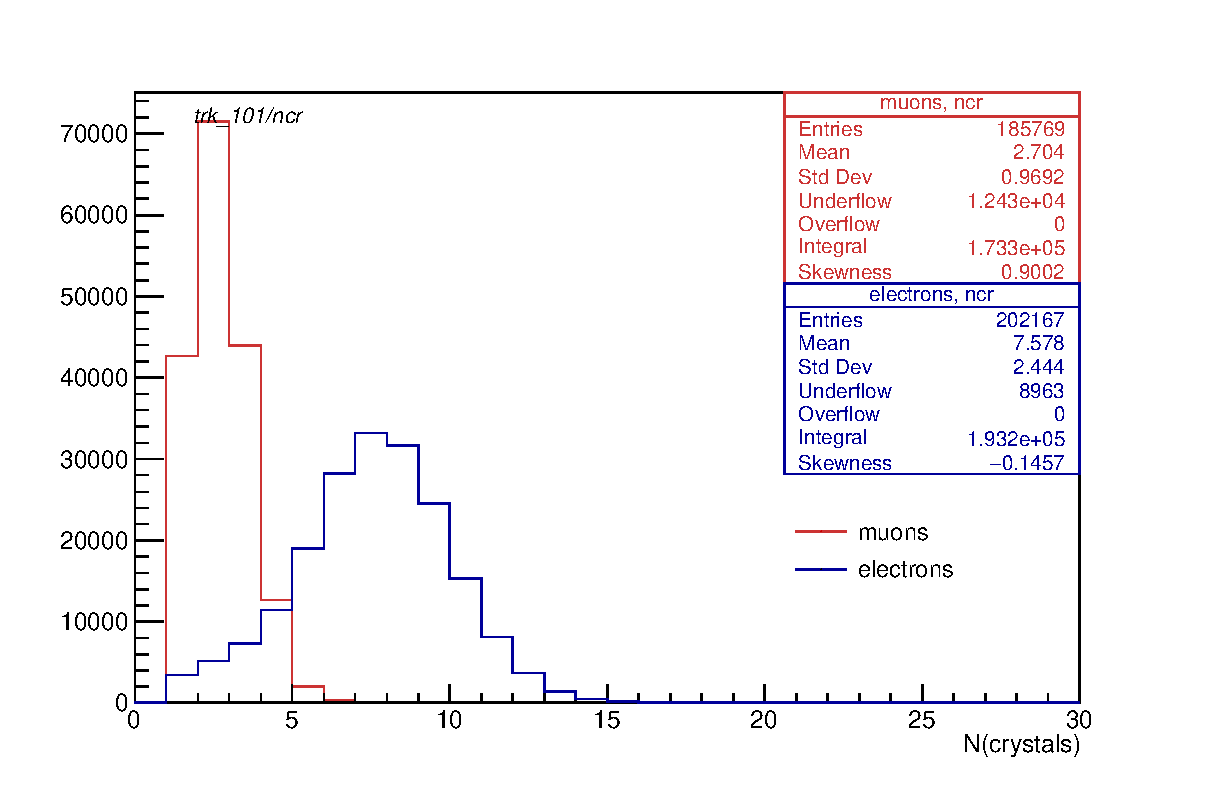
\includegraphics[width=0.50\textwidth]{figures/pdf/figure_00301_pid_emuana_1070_trk_101_ncr}
      % }
    };
    \node[anchor=south west,inner sep=0] at (-1,-6.) {
      % \node[shift={(0 cm,0.cm)},inner sep=0,rotate={90}] at (0,0) {}
      % \makebox[\textwidth][c] {
      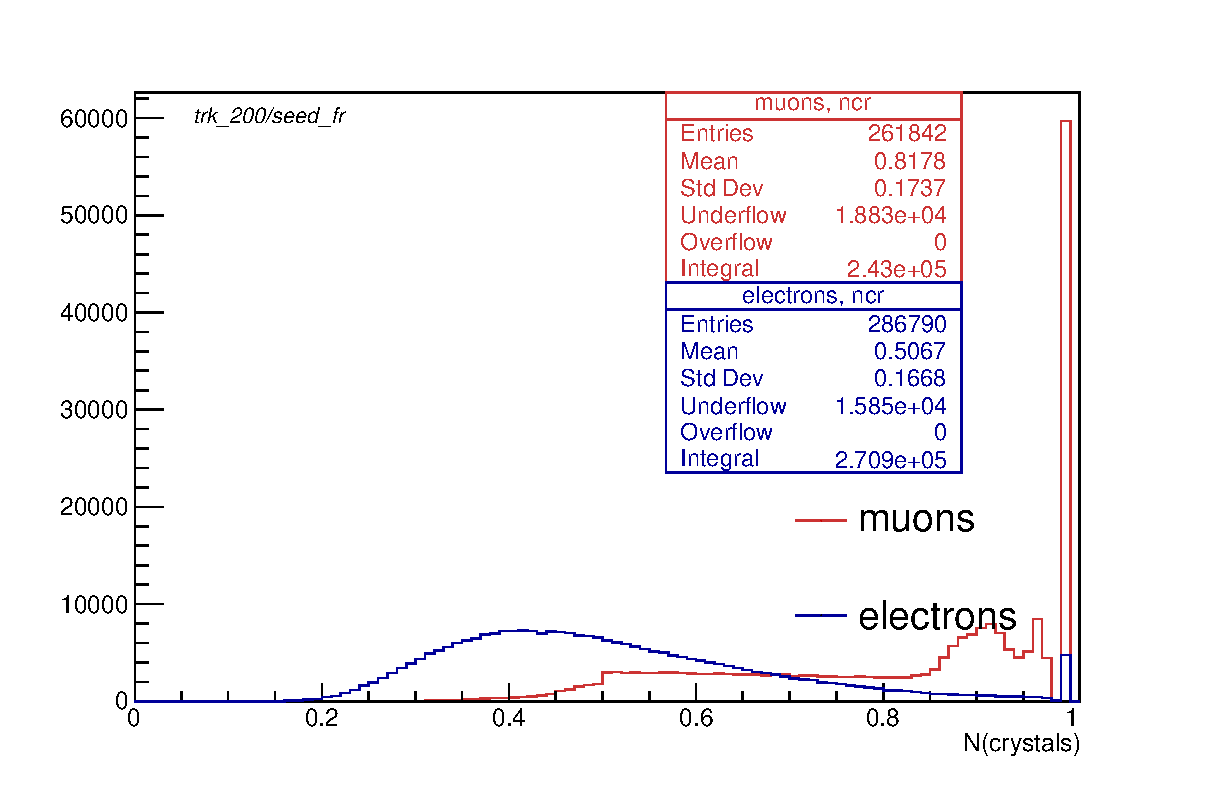
\includegraphics[width=0.50\textwidth]{figures/pdf/figure_00302_pid_emuana_1070_trk_101_seed_fr}
      % }
    };
    \node[anchor=south west,inner sep=0] at (9.5,-6.) {
      % \node[shift={(0 cm,0.cm)},inner sep=0,rotate={90}] at (0,0) {}
      % \makebox[\textwidth][c] {
      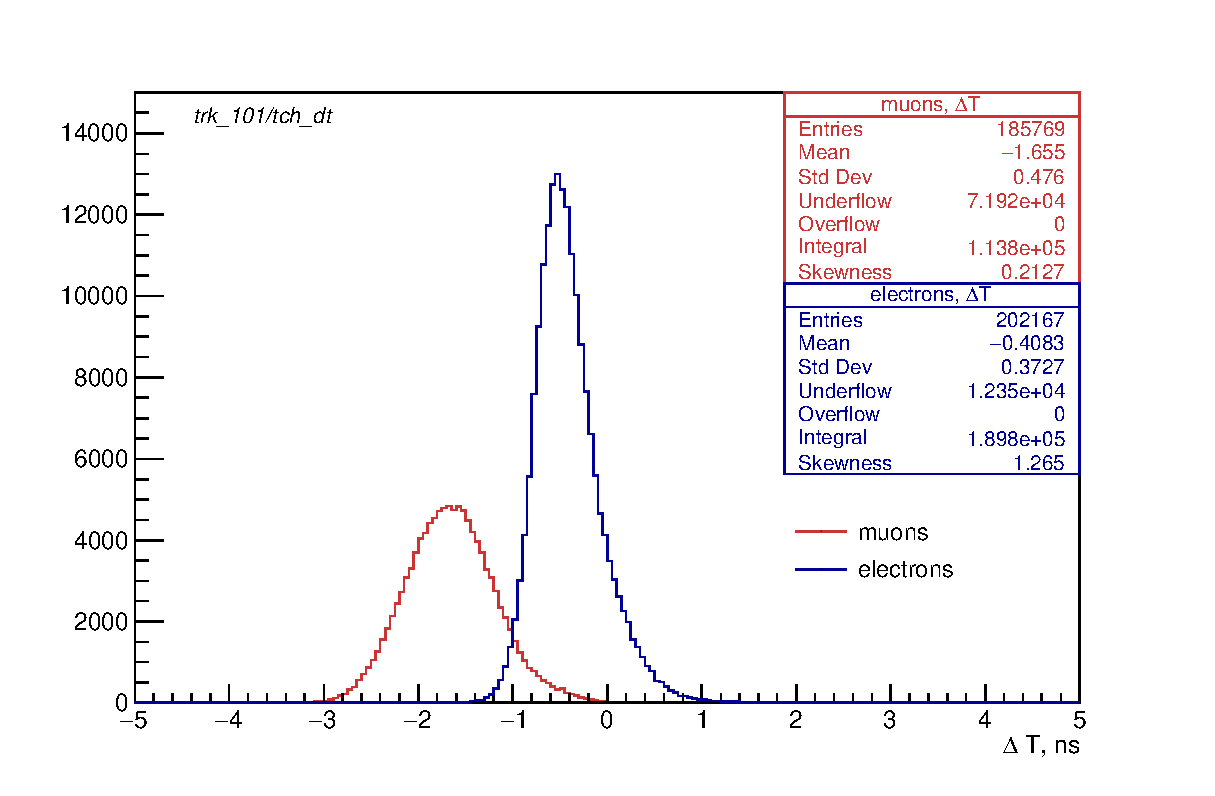
\includegraphics[width=0.50\textwidth]{figures/pdf/figure_00303_pid_emuana_1070_trk_101_tch_dt}
      % }
    };
    % \node [text width=6cm, scale=0.8] at (4.5,6.4) {mu2e-18894 by Kevin Lynch and Jim Popp};
  \end{tikzpicture}
  % \captionof{figure} {
  \caption{
    \label{fig:pid_training_1}
    variables used in PID MVA training: E/P, N(crystals), E(seed)/E, $\Delta T$
  }
\end{figure}

%%%%%%%%%% another figure
\begin{figure}[H]
  \hspace{-0.6in}
  \begin{tikzpicture}
    \node[anchor=south west,inner sep=0] at (0,0.) {
      % \node[shift={(0 cm,0.cm)},inner sep=0,rotate={90}] at (0,0) {}
      % \makebox[\textwidth][c] {
      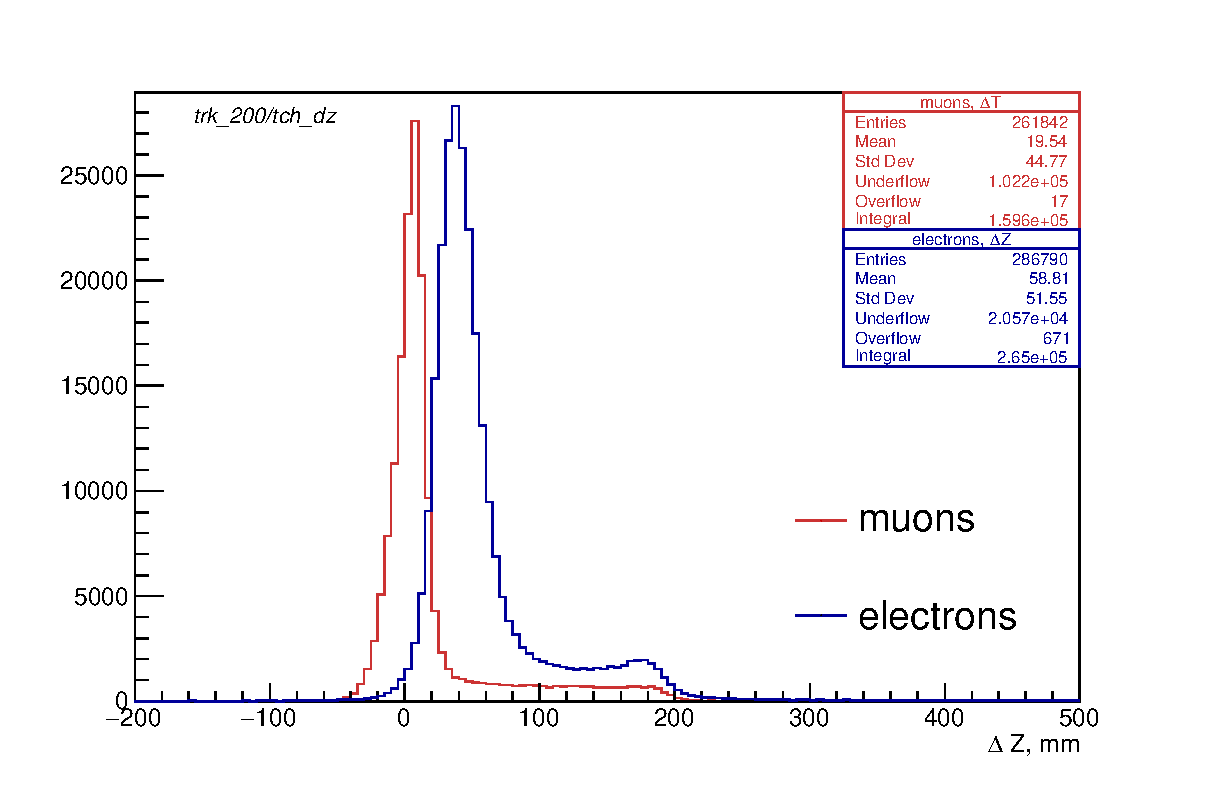
\includegraphics[width=0.50\textwidth]{figures/pdf/figure_00304_pid_emuana_1070_trk_101_tch_dz}
      % }
    };
    \node[anchor=south west,inner sep=0] at (10.5,0) {
      % \node[shift={(0 cm,0.cm)},inner sep=0,rotate={90}] at (0,0) {}
      % \makebox[\textwidth][c] {
      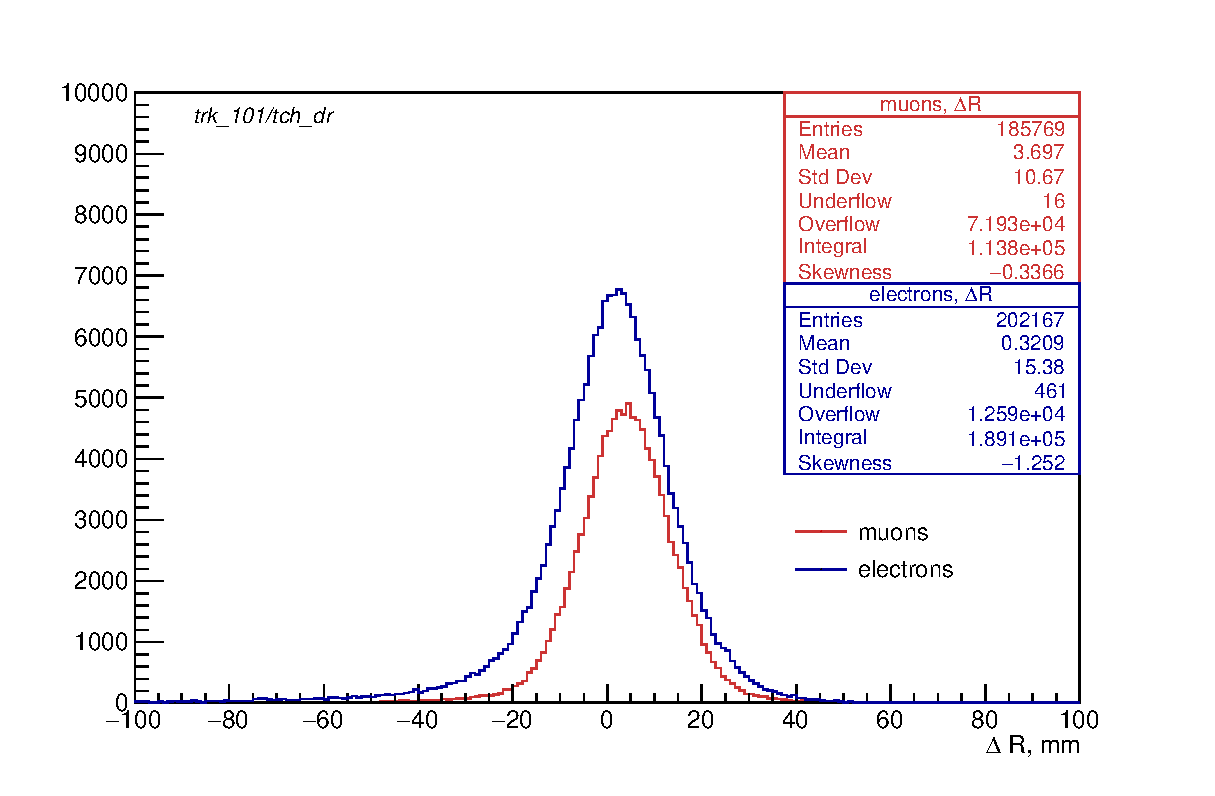
\includegraphics[width=0.50\textwidth]{figures/pdf/figure_00305_pid_emuana_1070_trk_101_tch_dr}
      % }
    };
    \node[anchor=south west,inner sep=0] at (0.,-6) {
      % \node[shift={(0 cm,0.cm)},inner sep=0,rotate={90}] at (0,0) {}
      % \makebox[\textwidth][c] {
      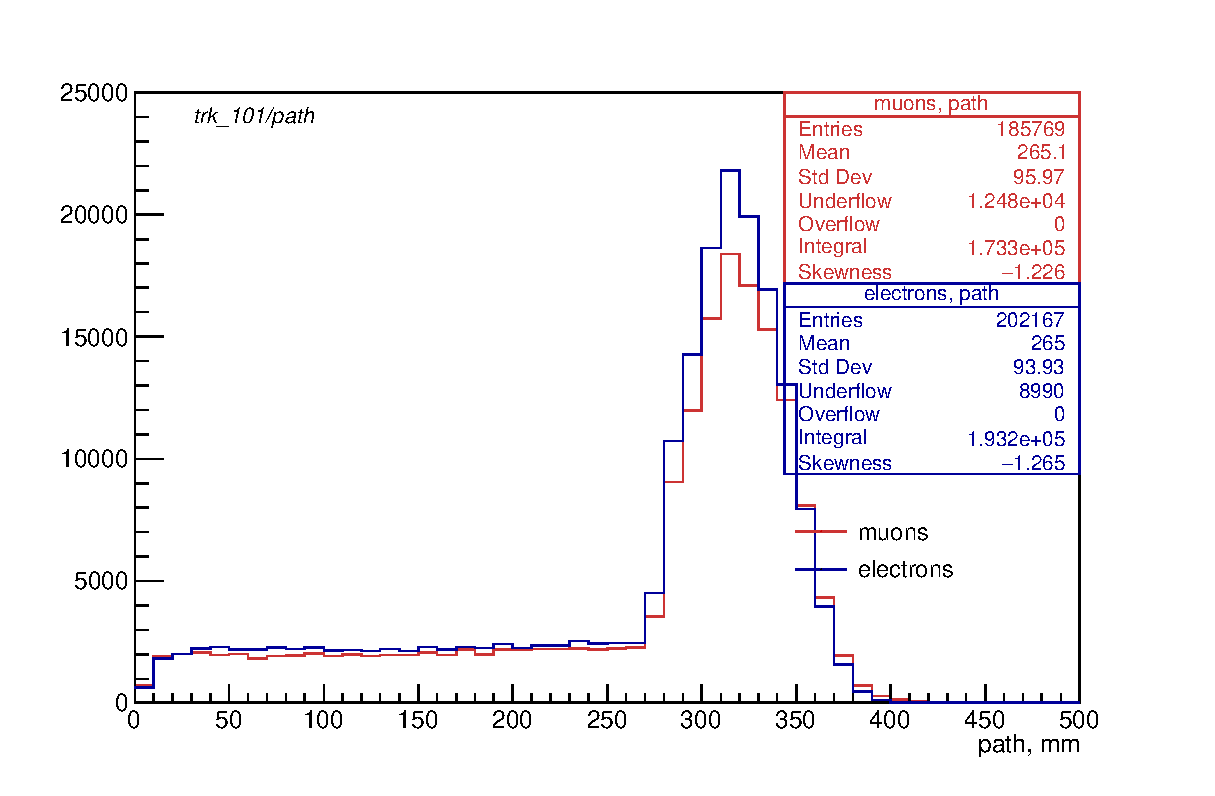
\includegraphics[width=0.50\textwidth]{figures/pdf/figure_00306_pid_emuana_1070_trk_101_path}
      % }
    };
    % \node [text width=6cm, scale=0.8] at (4.5,6.4) {mu2e-18894 by Kevin Lynch and Jim Popp};
  \end{tikzpicture}
  \captionof{figure} {
    % \caption{
    \label{fig:pid_training_2}
    variables used in PID MVA training: $\Delta Z$, $\Delta R$, path
  }
\end{figure}


Results of the PID ANN training are shown in Figure \ref{fig:pid_training_3}. 
From the training plots, one might conclude that the separation between the
electrons and muons provided by the ANN is close to perfect. 

To identify 105 MeV electrons, we require the PID ANN score $S_{PID} > 0.5$.

\begin{figure}[H]
\hspace{-0.6in}
  \begin{tikzpicture}
    \node[anchor=south west,inner sep=0] at (0,0.) {
      % \node[shift={(0 cm,0.cm)},inner sep=0,rotate={90}] at (0,0) {}
      % \makebox[\textwidth][c] {
      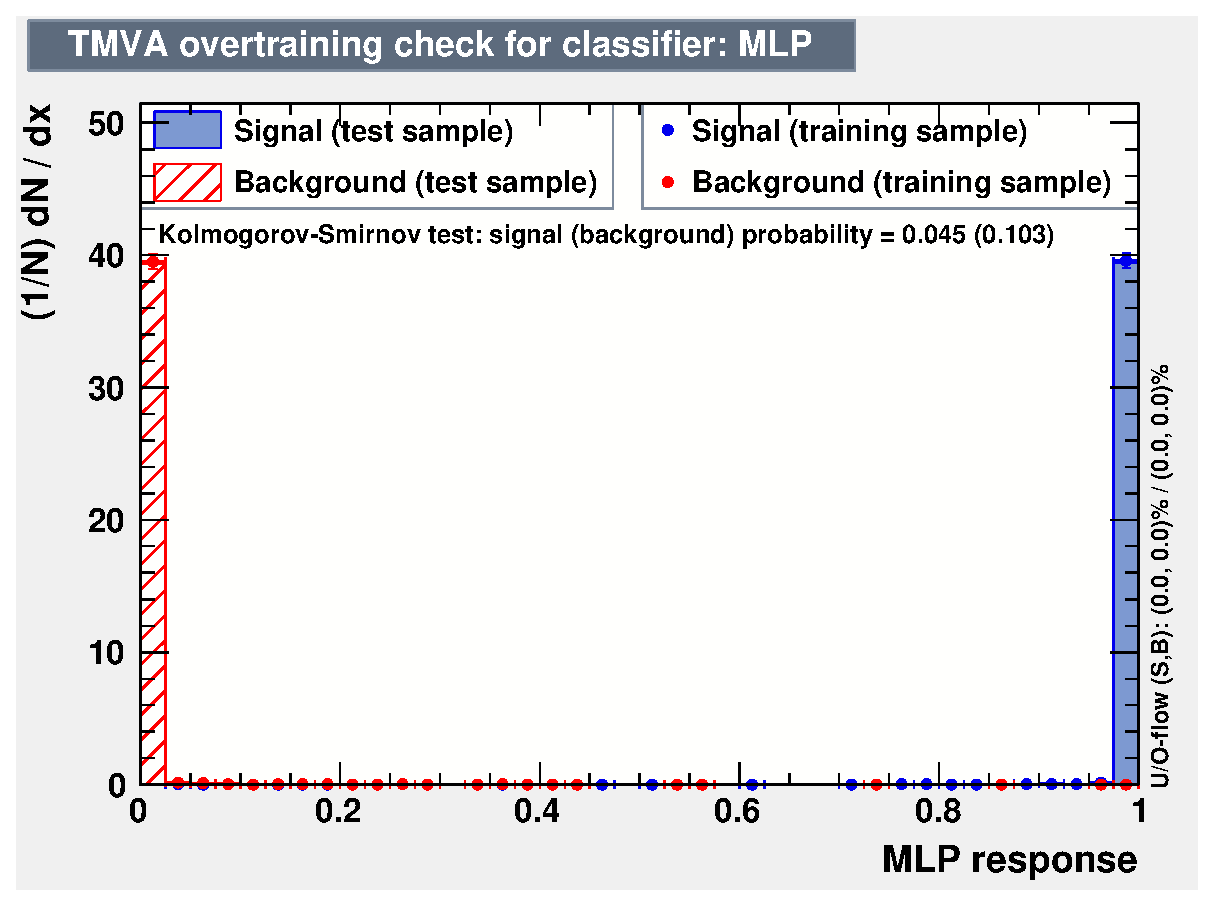
\includegraphics[width=0.55\textwidth]{figures/pdf/pid_mva_overtrain_mlp}
      % }
    };
    \node[anchor=south west,inner sep=0] at (10.5,0.5) {
      % \node[shift={(0 cm,0.cm)},inner sep=0,rotate={90}] at (0,0) {}
      % \makebox[\textwidth][c] {
      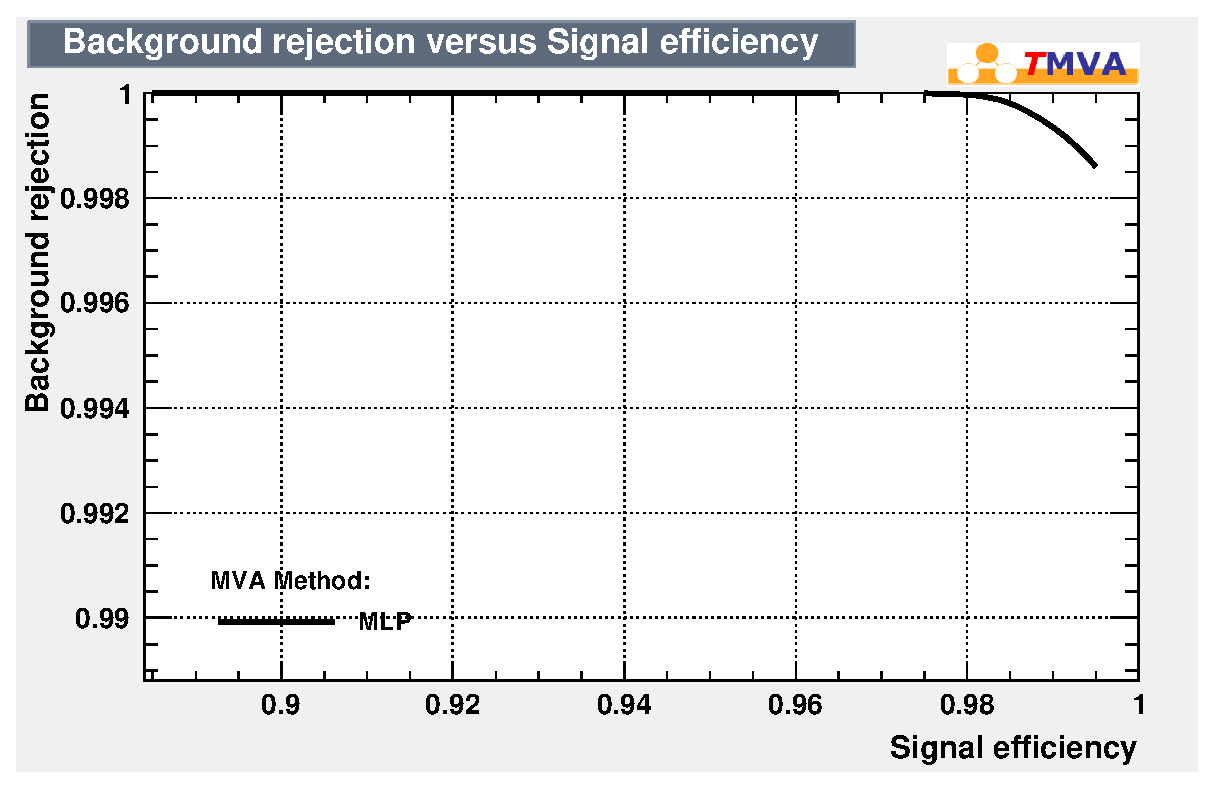
\includegraphics[width=0.55\textwidth]{figures/pdf/pid_mva_rejection_mlp}
      % }
    };
    % \node [text width=6cm, scale=0.8] at (4.5,6.4) {mu2e-18894 by Kevin Lynch and Jim Popp};
  \end{tikzpicture}
  % \captionof{figure} {
  \caption{
    \label{fig:pid_training_3}
    output of the PID ANN training: overtraining check on the left and efficiency vs rejection 
    on the right
  }
\end{figure}

PID ANN training is validated by running the PID algorithm on full ele00s61b0 and mumi0s51b0 datasets.
The datasets have about 200K events each, including events used for training. 
Results presented in Figure \ref{fig:pid_training_4} show that the efficiency of the $S_{PID} > 0.5$ cut 
for electrons is about 99.2\%, and about 0.8\% of muons are mis-identified as electrons. The spike at 1
in the ANN score distribution for muons corresponds to muon decays in flight, where the particle
reconstructed in the event is an electron. Remaining sources of muon mis-identification will be 
studied in detail later.

\begin{figure}[H]
  \begin{tikzpicture}
    \node[anchor=south west,inner sep=0] at (0,0.) {
      % \node[shift={(0 cm,0.cm)},inner sep=0,rotate={90}] at (0,0) {}
      \makebox[\textwidth][c] {
        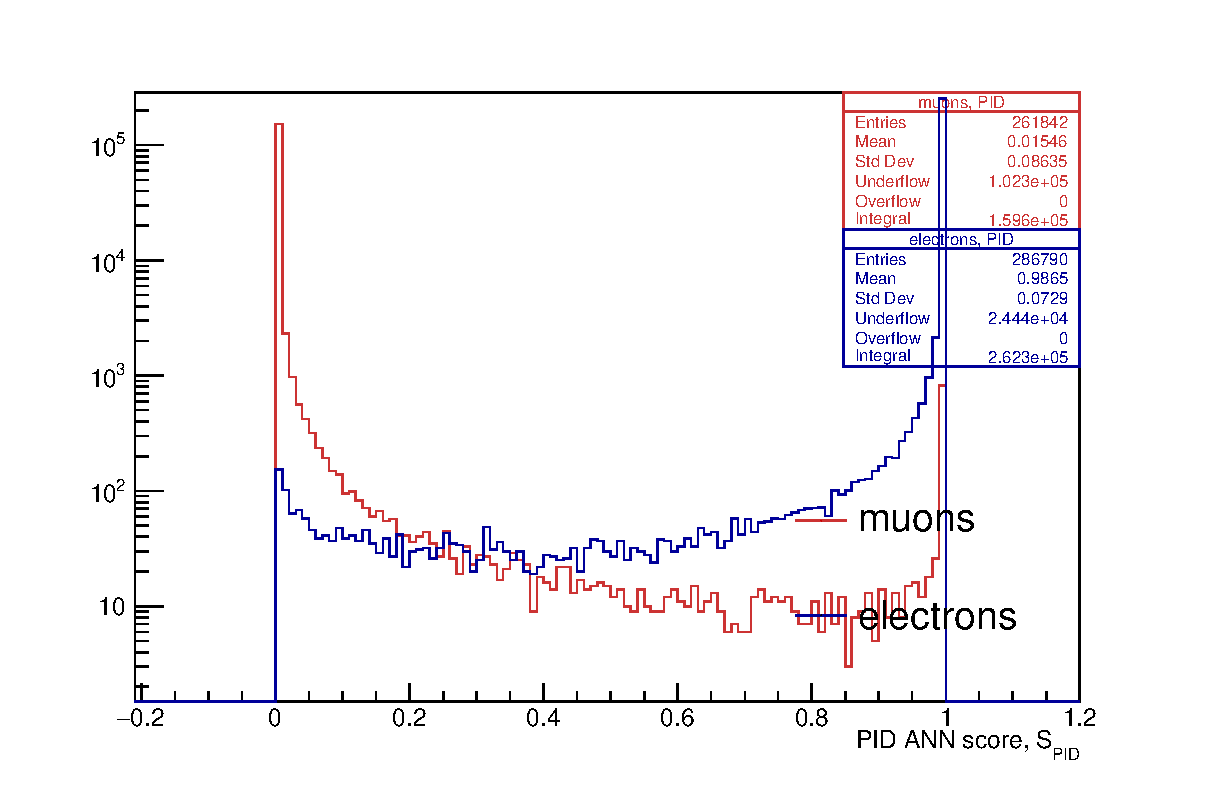
\includegraphics[width=1.0\textwidth]{figures/pdf/figure_00307_pid_emuana_1070_trk_101_pidmvaout}
      }
    };
    % \node [text width=6cm, scale=0.8] at (4.5,6.4) {mu2e-18894 by Kevin Lynch and Jim Popp};
  \end{tikzpicture}
  % \captionof{figure} {
  \caption{
    \label{fig:pid_training_4}
    Distribution in the PID ANN score for electron and muon samples, samples include events used for training,
    10000 events each. A spike in muon PID at 1  - muon decays in flight. \\ 
    {\color{red} \bf check that underflows are events without clusters}
  }
\end{figure}

Efficiencies of the PID preselection cuts for {\bf cele0s61b1} dataset are listed
in Table \ref{tab:pid_preselection_cuts}. The total preselection efficiency is about 93\%.
%
Out of that, approximately, 96\% comes from the requirement for the calorimeter cluster E > 10 MeV to be reconstructed in an event.
Therefore, for events with the reconstructed track with P>100 and a reconstructed cluster, efficiency
of the PID preselection is 0.967. Incremental efficiency of the PID selection is 0.993.

\begin{table}[H]
  \begin{center}
    \begin{tabular}{l|c|c} % <-- Changed to S here.
      \textbf{Cut}                    & \textbf{N events after } & \textbf{Efficiency }\\
      \hline
      Number generated events         & 1000000          &            \\
      total number of tracks          &  329715          &   0.330    \\
      \hline
      track passes TID cuts           &  193252          &   0.586    \\
      $P > 100$                       &  178078          &   0.921    \\
      $|DR| < 100$ mm                 &  167028          &   0.938    \\
      $|DT| < 10$ ns                  &  167028          &   1.0      \\
      $-50 < dz < 250$                &  164951          &   0.988    \\
      $ E/P < 1.2$                    &  164884          &   1.000    \\
      \hline
      $PID >0.5$                      &  163543          &   0.992    \\
   \end{tabular}
  \end{center}
  \caption{
    \label{tab:pid_preselection_cuts}
    PID preselection cuts (ele00s61b0) and efficiency for {\bf cele0s51b1} electrons 
  }
\end{table}

Out of 109004 muons $P > 100$ and passing the preselection cuts, 799 have the PID ANN score $S_{PID} > 0.5$,
which corresponds to the fake rate of about 0.8\%. Contributing to muon mis-identification are decays of
stopped muons in the calorimeter with muons decaying fast and the energy of the produced electron counted
as the part of the muon cluster energy. 


%%%%%%%%%%%%%%%%%%%%%%%%%%%%%%%%%%%%%%%%%%%%%%%%%%%%%%%%%%%%%%%%%%%%%%%%%%%%%%
\subsection { Electrons, failing the PID selection}
\label{sec:electrons_failing_pid}

Figure \ref{fig:electrons_failing_pid} compares distributions in some ID variables for electrons 
passing and failing the PID cuts.

Although only 0.8\% Of events are in question, understanding of the ANN failures could help finding 
reconstruction problems.
\begin{itemize}
\item 
  {\red Of special interest seems to be the spike in the distribution in $R_{max}$ - to be investigated}
\item
  {\red also electrons with $\Delta{T} < -1.5$ ns - to be investigated}
\end{itemize}

\begin{figure}[H]
\hspace{-0.6in}
  \begin{tikzpicture}
    \node[anchor=south west,inner sep=0] at (0,0.) {
      % \node[shift={(0 cm,0.cm)},inner sep=0,rotate={90}] at (0,0) {}
      % \makebox[\textwidth][c] {
      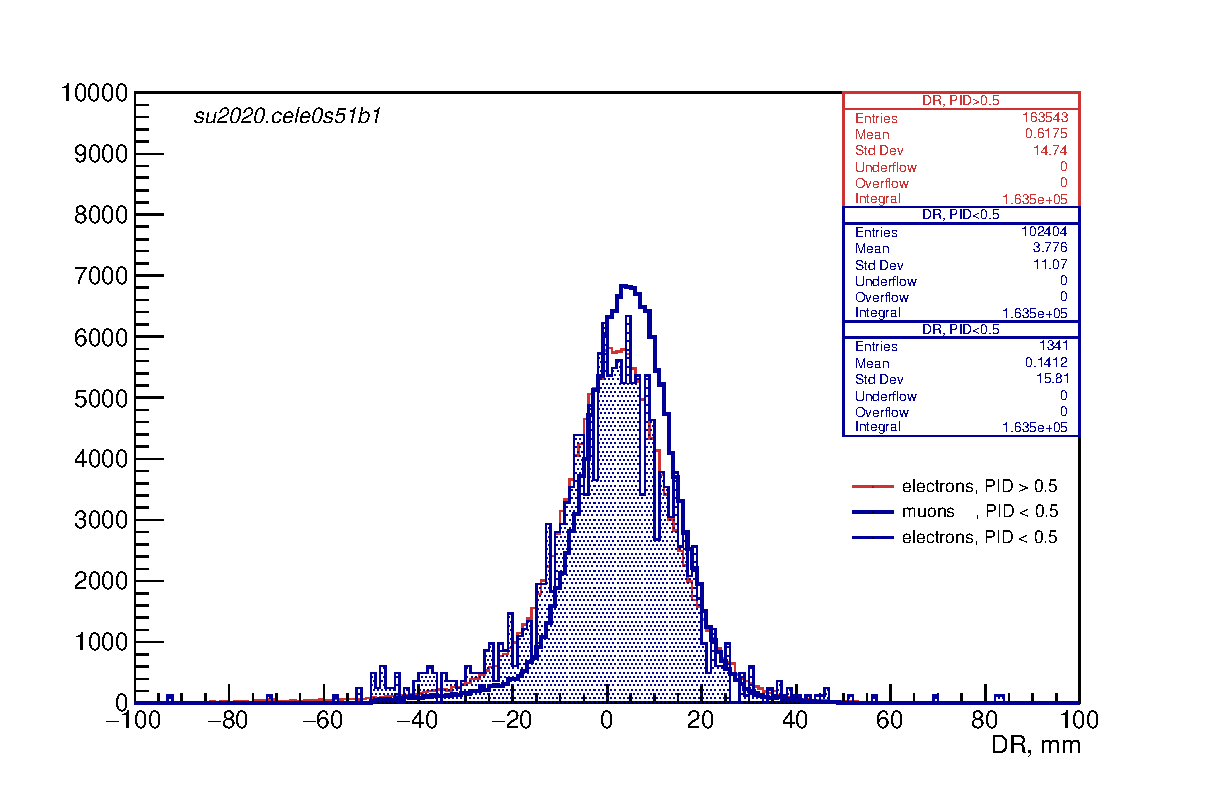
\includegraphics[width=0.60\textwidth]{figures/pdf/figure_00310_pid_emuana_trk_110_vs_111_tch_dr}
      % }
    };
    \node[anchor=south west,inner sep=0] at (10.3,0.) {
      % \node[shift={(0 cm,0.cm)},inner sep=0,rotate={90}] at (0,0) {}
      % \makebox[\textwidth][c] {
      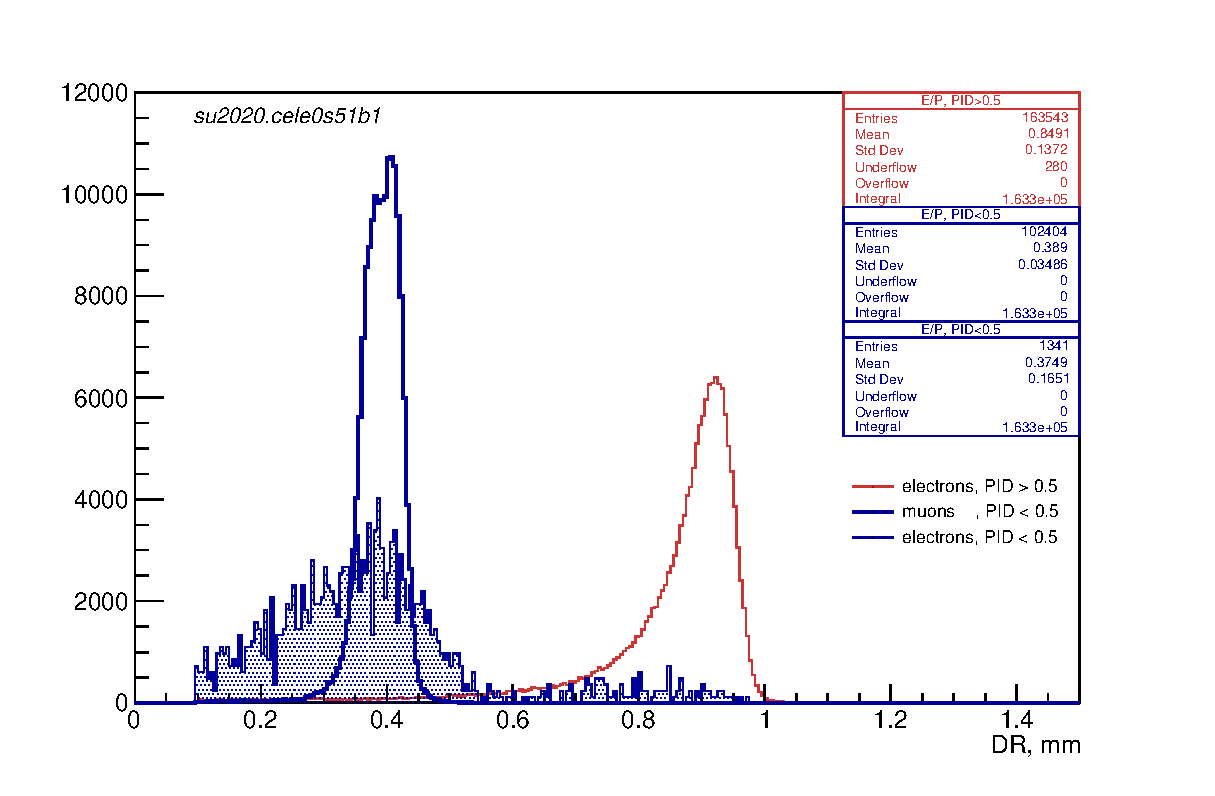
\includegraphics[width=0.60\textwidth]{figures/pdf/figure_00311_pid_emuana_trk_110_vs_111_ep}
      % }
    };
    \node[anchor=south west,inner sep=0] at (0,-7.0) {
      % \node[shift={(0 cm,0.cm)},inner sep=0,rotate={90}] at (0,0) {}
      % \makebox[\textwidth][c] {
      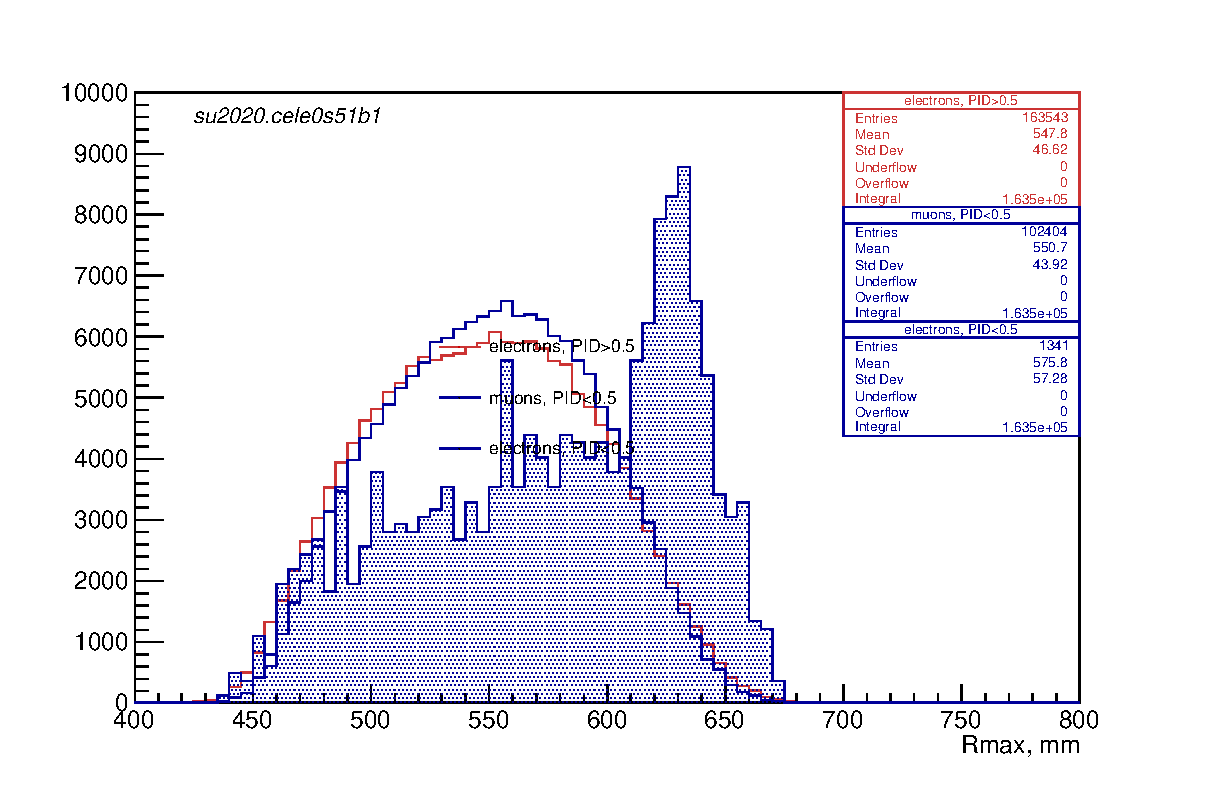
\includegraphics[width=0.60\textwidth]{figures/pdf/figure_00312_pid_emuana_trk_110_vs_111_rmax}
      % }
    };
    \node[anchor=south west,inner sep=0] at (10.3,-7.0) {
      % \node[shift={(0 cm,0.cm)},inner sep=0,rotate={90}] at (0,0) {}
      % \makebox[\textwidth][c] {
      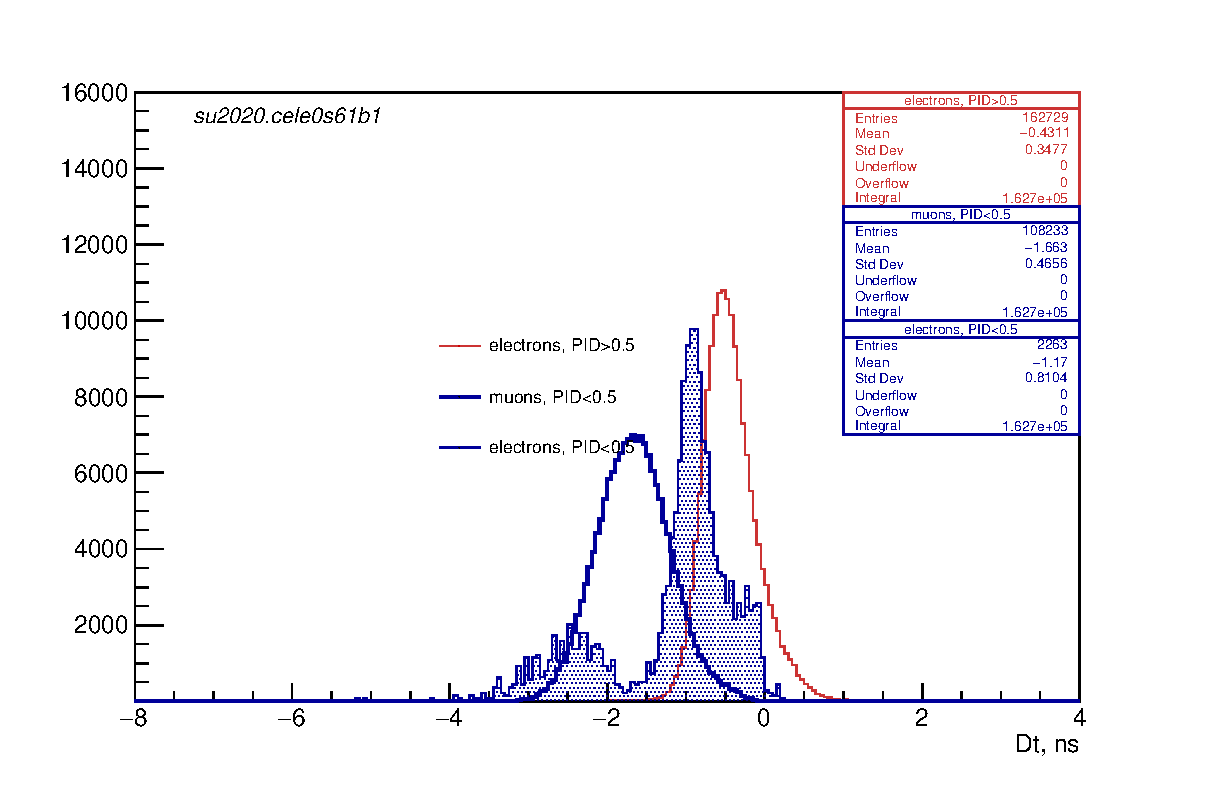
\includegraphics[width=0.60\textwidth]{figures/pdf/figure_00313_pid_emuana_trk_110_vs_111_tch_dt}
      % }
    };
    % \node [text width=6cm, scale=0.8] at (4.5,6.4) {mu2e-18894 by Kevin Lynch and Jim Popp};
  \end{tikzpicture}
  \captionof{figure} {
    \label{fig:electrons_failing_pid}
    % \caption{
    Distributions of the PID variables for electrons passing the PID, muons failing the PID, and electrons failing the PID.
    The PID selection used is $S_{PID} > 0.5$, where $S_{PID}$ is the value of the PID ANN score variable
  }
\end{figure}


%%%%%%%%%%%%%%%%%%%%%%%%%%%%%%%%%%%%%%%%%%%%%%%%%%%%%%%%%%%%%%%%%%%%%%%%%%%%%%
\newpage
\subsection{\MuToEp\ Channel}
\label{sec:mumep_channel_pid}

PID in \MuToEp\ channel uses a similar ANN trained  using  92 MeV/c positrons and$\mu^+$'s from {\bf pos01s51b0}
and {\bf mupl1s51b0} datasets. The training procedure is the same as described in Section \ref{sec:mumem_pid_ann_training}.
% 
Figure \ref{fig:pid_score_mumep} shows distributions of the PID ANN score, $S_{PID}$,
for 92 MeV positrons and $\mu^+$'s. About 1.2\% of all muon events have $S_{PID} > 0.5$,
more than 50\% of those events are electrons produced in muon decays in flight.

Plotting the data in log scale - see Figure \ref{fig:pid_score_mumep}(b) - reveals a spike around 0.25,
present in both positron and muon distributions.

{\red Although the relative contribution of the spike is small, its origin needs to be investigated.}

\begin{figure}[H]
\hspace{-0.6in}
  \begin{tikzpicture}
    \node[anchor=south west,inner sep=0] at (0,0.) {
      % \node[shift={(0 cm,0.cm)},inner sep=0,rotate={90}] at (0,0) {}
      % \makebox[\textwidth][c] {
      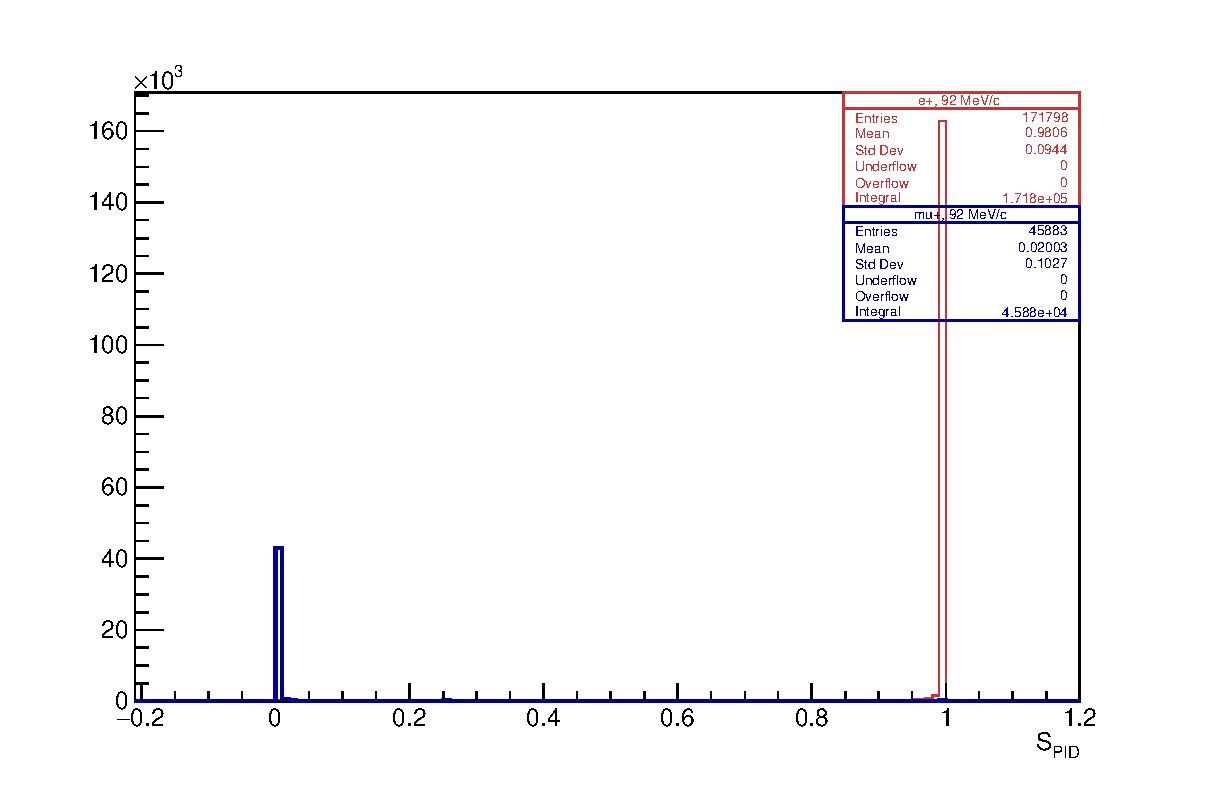
\includegraphics[width=0.60\textwidth]{figures/pdf/figure_00331_su2020_track_ana_1110_trk_219_pidmvaout}
      % }
    };
    \node [text width=1cm, scale=1.0] at (3.,4.5) {(a)};
    \node[anchor=south west,inner sep=0] at (10.5,0.) {
      % \node[shift={(0 cm,0.cm)},inner sep=0,rotate={90}] at (0,0) {}
      % \makebox[\textwidth][c] {
      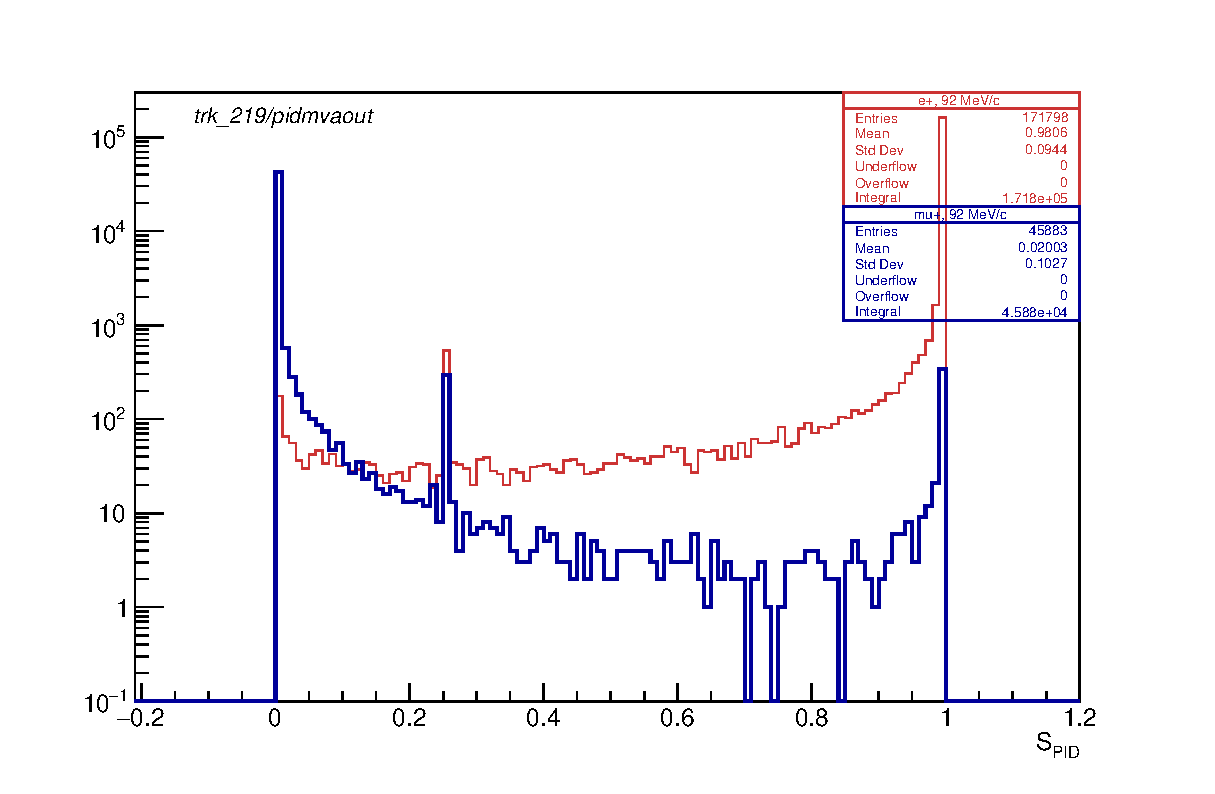
\includegraphics[width=0.60\textwidth]{figures/pdf/figure_00332_su2020_track_ana_1110_trk_219_pidmvaout_log}
      % }
    };
    \node [text width=1cm, scale=1.0] at (13.5,4.5) {(b)};
  \end{tikzpicture}
  \captionof{figure} {
    \label{fig:pid_score_mumep}
    Results of the PID ANN training for \MuToEp\ channel: distribution of the PID ANN score, $S_{PID}$,
    for single 92.3 positrons and positive muons; (a): linear scale; (b): log scale.
    {\red Nature of the spike around 0.25 needs to be investigated.}
  }
\end{figure}